% Options for packages loaded elsewhere
\PassOptionsToPackage{unicode}{hyperref}
\PassOptionsToPackage{hyphens}{url}
%
\documentclass[
]{book}
\usepackage{lmodern}
\usepackage{amssymb,amsmath}
\usepackage{ifxetex,ifluatex}
\ifnum 0\ifxetex 1\fi\ifluatex 1\fi=0 % if pdftex
  \usepackage[T1]{fontenc}
  \usepackage[utf8]{inputenc}
  \usepackage{textcomp} % provide euro and other symbols
\else % if luatex or xetex
  \usepackage{unicode-math}
  \defaultfontfeatures{Scale=MatchLowercase}
  \defaultfontfeatures[\rmfamily]{Ligatures=TeX,Scale=1}
\fi
% Use upquote if available, for straight quotes in verbatim environments
\IfFileExists{upquote.sty}{\usepackage{upquote}}{}
\IfFileExists{microtype.sty}{% use microtype if available
  \usepackage[]{microtype}
  \UseMicrotypeSet[protrusion]{basicmath} % disable protrusion for tt fonts
}{}
\makeatletter
\@ifundefined{KOMAClassName}{% if non-KOMA class
  \IfFileExists{parskip.sty}{%
    \usepackage{parskip}
  }{% else
    \setlength{\parindent}{0pt}
    \setlength{\parskip}{6pt plus 2pt minus 1pt}}
}{% if KOMA class
  \KOMAoptions{parskip=half}}
\makeatother
\usepackage{xcolor}
\IfFileExists{xurl.sty}{\usepackage{xurl}}{} % add URL line breaks if available
\IfFileExists{bookmark.sty}{\usepackage{bookmark}}{\usepackage{hyperref}}
\hypersetup{
  pdftitle={An Introduction to Data Science for Sensory and Consumer Scientists},
  pdfauthor={John Ennis, Julien Delarue, and Thierry Worch},
  hidelinks,
  pdfcreator={LaTeX via pandoc}}
\urlstyle{same} % disable monospaced font for URLs
\usepackage{longtable,booktabs}
% Correct order of tables after \paragraph or \subparagraph
\usepackage{etoolbox}
\makeatletter
\patchcmd\longtable{\par}{\if@noskipsec\mbox{}\fi\par}{}{}
\makeatother
% Allow footnotes in longtable head/foot
\IfFileExists{footnotehyper.sty}{\usepackage{footnotehyper}}{\usepackage{footnote}}
\makesavenoteenv{longtable}
\usepackage{graphicx}
\makeatletter
\def\maxwidth{\ifdim\Gin@nat@width>\linewidth\linewidth\else\Gin@nat@width\fi}
\def\maxheight{\ifdim\Gin@nat@height>\textheight\textheight\else\Gin@nat@height\fi}
\makeatother
% Scale images if necessary, so that they will not overflow the page
% margins by default, and it is still possible to overwrite the defaults
% using explicit options in \includegraphics[width, height, ...]{}
\setkeys{Gin}{width=\maxwidth,height=\maxheight,keepaspectratio}
% Set default figure placement to htbp
\makeatletter
\def\fps@figure{htbp}
\makeatother
\setlength{\emergencystretch}{3em} % prevent overfull lines
\providecommand{\tightlist}{%
  \setlength{\itemsep}{0pt}\setlength{\parskip}{0pt}}
\setcounter{secnumdepth}{5}
\usepackage{booktabs}
\ifluatex
  \usepackage{selnolig}  % disable illegal ligatures
\fi
\usepackage[]{natbib}
\bibliographystyle{apalike}

\title{An Introduction to Data Science for Sensory and Consumer Scientists}
\author{John Ennis, Julien Delarue, and Thierry Worch}
\date{2020-12-29}

\begin{document}
\maketitle

{
\setcounter{tocdepth}{1}
\tableofcontents
}
\hypertarget{preface}{%
\chapter*{Preface}\label{preface}}
\addcontentsline{toc}{chapter}{Preface}

Welcome to the website for \emph{Introduction to Data Science for Sensory and Consumer Scientists}. This book being written in the open and is currently under development.

\hypertarget{about-the-authors}{%
\chapter*{About the Authors}\label{about-the-authors}}
\addcontentsline{toc}{chapter}{About the Authors}

John Ennis \ldots{}

Julien Delarue \ldots{}

Thierry Worch \ldots{}

\hypertarget{part-introduction}{%
\part*{Introduction}\label{part-introduction}}
\addcontentsline{toc}{part}{Introduction}

\hypertarget{intro}{%
\chapter{Introduction}\label{intro}}

Sensory and consumer science (SCS) is consider as a pillar of food science and technology and is useful to product development, quality control and market research. Most scientific and methodological advances in the field are applied to food. This book makes no exception as we chose a cookie formulation dataset as a main thread. However, SCS widely applies to many other consumer goods so are the content of this book and the principles set out below.

\hypertarget{core-principles-in-sensory-and-consumer-science}{%
\section{Core principles in Sensory and Consumer Science}\label{core-principles-in-sensory-and-consumer-science}}

\hypertarget{measuring-and-analyzing-human-responses}{%
\subsection{Measuring and analyzing human responses}\label{measuring-and-analyzing-human-responses}}

Sensory and consumer science aims at measuring and understanding consumers' sensory perceptions as well as the judgements, emotions and behaviors that may arise from these perceptions. SCS is thus primarily a science of measurement, although a very particular one that uses human beings and their senses as measuring instruments. In other words, sensory and consumer researchers measure and analyze human responses.
To this end, SCS relies essentially on sensory evaluation which comprises a set of techniques that mostly derive from psychophysics and behavioral research. It uses psychological models to help separate signal from noise in collected data {[}ref O'Mahony, D.Ennis, others?{]}. Besides, sensory evaluation has developed its own methodological framework that includes most refined techniques for the accurate measurement of product sensory properties while minimizing the potentially biasing effects of brand identity and the influence of other external information on consumer perception {[}Lawless \& Heymann, 2010{]}.
A detailed description of sensory methods is beyond the scope of this book and many textbooks on sensory evaluation methods are available to readers seeking more information. However, just to give a brief overview, it is worth remembering that sensory methods can be roughly divided into three categories, each of them bearing many variants:
- Discrimination tests that aim at detecting subtle differences between two products.
- Descriptive analysis (DA), also referred to as `sensory profiling', aims at providing both qualitative and quantitative information about product sensory properties.
- Hedonic tests. This category gathers affective tests that aim at measuring consumers' liking for the tested products or their preferences among a product set.
Each of these test categories generates its own type of data and related statistical questions in relation to the objectives of the study. Typically, data from difference tests consist in series of correct/failed binary answers depending on whether judges successfully picked the odd sample(s) among a set of three or more samples. These are used to determine whether the number of correct choices is above the level expected by chance.
Conventional descriptive analysis data consist in intensity scores given by each panelist to evaluated samples on a series of sensory attributes, hence resulting in a product x attribute x panelist dataset (Figure 1). Note that depending on the DA method, quantifying means other than intensity ratings can be used (ranks, frequency, etc.). Most frequently, each panelist evaluates all the samples in the product set. However, the use of balanced incomplete design can also be found when the experimenters aim to limit the number of samples evaluated by each subject.
Eventually, hedonic test datasets consist in hedonic scores (ratings for consumers' degree of liking or preference ranks) given by each interviewed consumer to a series of products. As for DA, each consumer usually evaluates all the samples in the product set, but balanced incomplete designs are sometimes used too. In addition, some companies favor pure monadic evaluation of product (i.e.~between-subject design or independent groups design) which obviously result in unrelated sample datasets.
Sensory and consumer researchers also borrow methods from other fields, in particular from sociology and experimental psychology. Definitely a multidisciplinary area, SCS develops in many directions and reaches disciplines that range from genetics and physiology to social marketing, behavioral economics and computational neuroscience. So have diversified the types of data sensory and consumer scientists must deal with.

\hypertarget{how-should-sensory-and-consumer-scientists-learn-data-science}{%
\section{How should sensory and consumer scientists learn data science?}\label{how-should-sensory-and-consumer-scientists-learn-data-science}}

\hypertarget{caution-dont-that-everybody-does}{%
\section{Caution: Don't that everybody does}\label{caution-dont-that-everybody-does}}

\hypertarget{example-projects}{%
\section{Example projects}\label{example-projects}}

\hypertarget{data_science}{%
\chapter{What is Data Science?}\label{data_science}}

In this chapter we explain what is data science.

\hypertarget{history-and-definition}{%
\section{History and Definition}\label{history-and-definition}}

Data science has been called the ``sexiest job of the 21st century'' by Harvard Business Review {[}insert DJ Patil reference{]}, but what is it? As with all rapidly growing fields, the definition depends on who you ask. Before we give our definition, however, we provide a brief history for context.

To begin, we note that there was a movement in early computer science to call their field ``data science.'' Chief among the advocates for this viewpoint was Peter Naur, winner of the 2005 Turing award. This viewpoint is detailed in the preface to his 1974 book, ``Concise Survey of Computer Methods,'' where he states that data science is ``the science of dealing with data, once they have been established.'' From his perspective, this is the purpose of computer science. This viewpoint is echoed in the statement, often attributed to Edsger Dijkstr, that ``Computer science is no more about computers than astronomy is about telescopes.''

Interestingly, a similar movement arose in statistics, starting in 1962 with John Tukey's statements that ``Data analysis, and the parts of statistics which adhere to it, must \ldots{} take on the characteristics of science rather than those of mathematics'' and that ``data analysis is intrinsically an empirical science.'' This movement culminated in 1997 when Jeff Wu proposed during his inaugural lecture, upon becoming the chair of the University of Michigan's statistics department, that statistics should be called data science.

These two movements came together in 2001 in William S. Cleveland's paper ``Data Science: An Action Plan for Expanding the Technical Areas in the Field of Statistics.'' In this highly influential monograph, Cleveland makes the key assertion that ``The value of technical work is judged by the extent ot which it benefits the data analyst, either directly or indirectly.''

{[}FOOTNOTE: It is worth noting that these two movements were connected by substantial work in the areas of statistical computing, knowledge discovery, and data mining, with important work contributed by Gregory Piatetsky-Shapiro, Usama Fayyad, and Padhraic Smyth among many others.{]}

Putting this history together, we provide our definition of \textbf{data science} as: The intersection of statistics, computer science, and industrial design. Accordingly, we use the following three definitions of these fields:

\begin{itemize}
\tightlist
\item
  \textbf{Statistics}: The branch of mathematics dealing with the collection, analysis, interpretation, and presentation of masses of numerical data.
\item
  \textbf{Computer Science}: Computer science is the study of processes that interact with data and that can be represented as data in the form of programs.
\item
  \textbf{Industrial Design}: The professional service of creating and developing concepts and specifications that optimize the function, value, and appearance of products and systems for the mutual benefit of both user and manufacturer.
\end{itemize}

Hence data science is the production of useful things through the collection, processing, analysis, and interpretation of data.

\hypertarget{workflow}{%
\section{Workflow}\label{workflow}}

A schematic of a data scientific workflow is shown in Figure \ref{fig:ds-workflow}. Each section is described in greater detail below.

\begin{figure}

{\centering 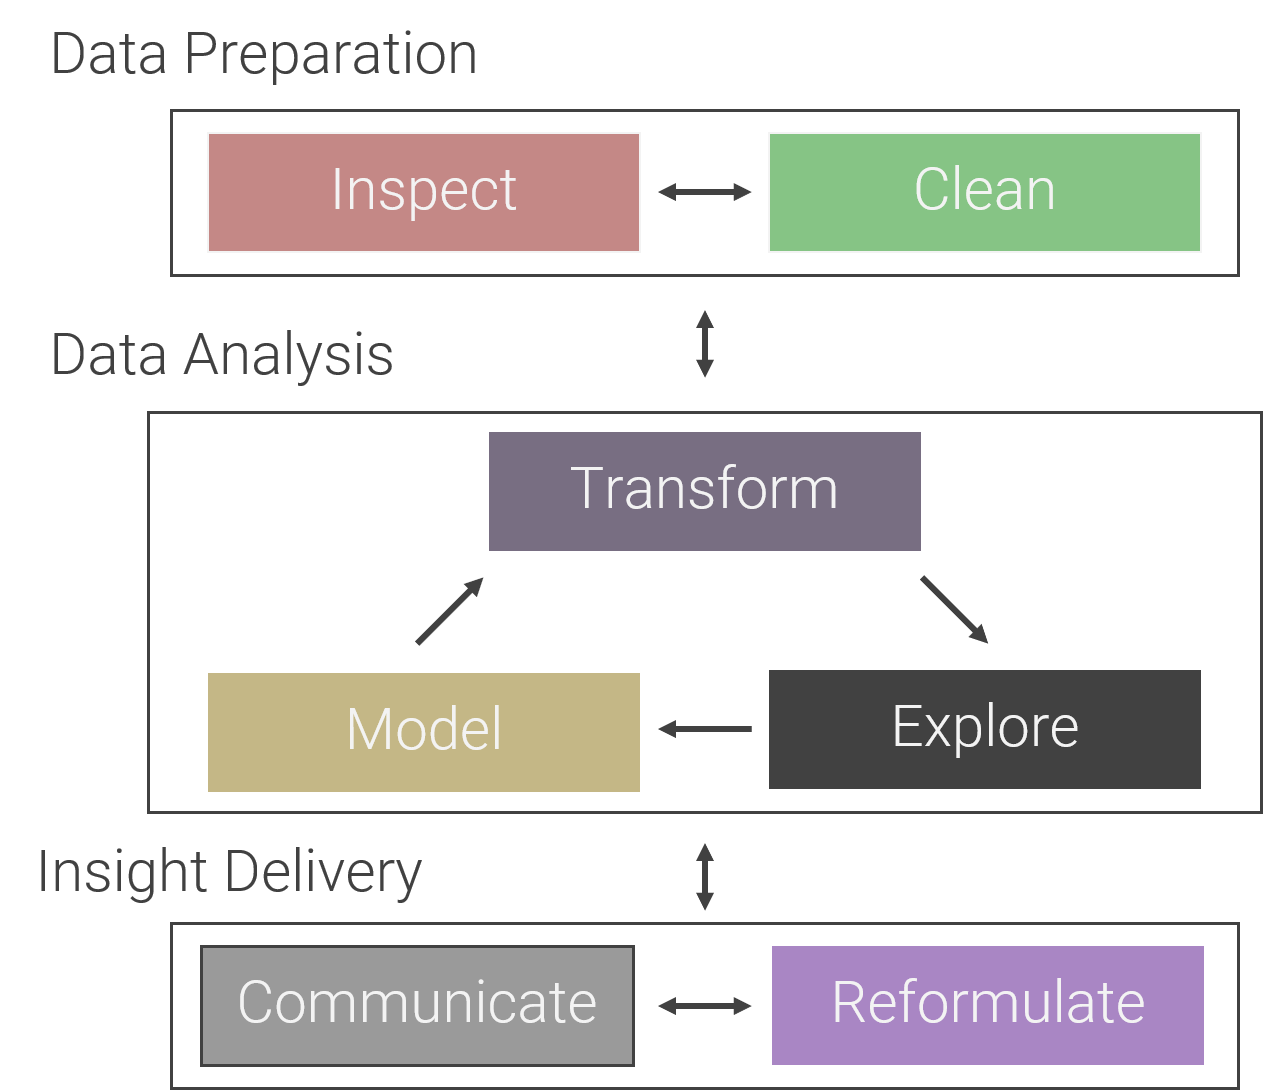
\includegraphics[width=17.54in]{images/data_science_workflow} 

}

\caption{Data scientific workflow.}\label{fig:ds-workflow}
\end{figure}

\hypertarget{data-preparation}{%
\subsection{Data Preparation}\label{data-preparation}}

\hypertarget{inspect}{%
\subsubsection{Inspect}\label{inspect}}

Goal:
Gain familiarity with the data
Key Steps:
Learn collection details
Check data imported correctly
Determine data types
Ascertain consistency and validity
Tabulate and compute other basic summary statistics
Create basic plots of key variables of interest

\hypertarget{clean}{%
\subsubsection{Clean}\label{clean}}

Goal:
Prepare data for analysis
Key Steps:
Remove/correct errors
Make data formatting consistent
Organize text data
Create tidy data (one observation per row)
Organize data into related tables
Document all choices

\hypertarget{data-analysis}{%
\subsection{Data Analysis}\label{data-analysis}}

\hypertarget{transform}{%
\subsubsection{Transform}\label{transform}}

Goal:
Adjust data as needed for analysis
Key Steps:
Create secondary variables
Decorrelate data
Identify latent factors
Engineer new features

\hypertarget{explore}{%
\subsubsection{Explore}\label{explore}}

Goal:
Allow data to suggest hypotheses
Key Steps:
Graphical visualizations
Exploratory analyses
Note:
Caution must be taken to avoid high false discovery rate when using automated tools

\hypertarget{model}{%
\subsubsection{Model}\label{model}}

Goal:
Conduct formal statistical modeling
Key Steps:
Conduct traditional statistical modeling
Build predictive models
Note:
This step may feed back into transform and explore

\hypertarget{insight-delivery}{%
\subsection{Insight Delivery}\label{insight-delivery}}

\hypertarget{communicate}{%
\subsubsection{Communicate}\label{communicate}}

Goal:
Exchange research information
Key Steps:
Automate reporting as much as possible
Share insights
Receive feedback
Note:
Design principles essential to make information accessible

\hypertarget{reformulate}{%
\subsubsection{Reformulate}\label{reformulate}}

Goal:
Incorporate feedback into workflow
Key Steps:
Investigate new questions
Revise communications
Note:
Reformulation make take us back to data cleaning

\hypertarget{benefits-of-data-science}{%
\section{Benefits of Data Science}\label{benefits-of-data-science}}

\hypertarget{reproducible-research}{%
\subsection{Reproducible Research}\label{reproducible-research}}

\begin{itemize}
\tightlist
\item
  Time savings
\item
  Collaboration
\item
  Continuous improvement
\end{itemize}

\hypertarget{data-driven-decision-making}{%
\subsection{Data-Driven Decision Making}\label{data-driven-decision-making}}

\hypertarget{standardized-data-collection}{%
\subsection{Standardized Data Collection}\label{standardized-data-collection}}

\hypertarget{standardized-reporting}{%
\subsection{Standardized Reporting}\label{standardized-reporting}}

\begin{itemize}
\tightlist
\item
  Especially valuable when there are multiple sites globally
\end{itemize}

\hypertarget{improved-business-impact}{%
\subsection{Improved Business Impact}\label{improved-business-impact}}

\hypertarget{how-to-learn-data-science}{%
\section{How to Learn Data Science}\label{how-to-learn-data-science}}

Learning data science is much like learning a language or learning to play an instrument - you have to practice. Our advice based on mentoring many students and clients is to get started sooner rather than later, and to accept that the code you'll write in the future will always be better than the code you'll write today. Also, many of the small details that separate an proficient data scientist from a novice can only really be learned through practice as there are too many small details to learn them all in advice. So, starting today, do your best to write at least some code for all your projects. If a time deadline prevents you from completing the analysis in R, that's fine, but at least gain the experience of making an RStudio project and loading the data in R. Then, as time allows, try to duplicate your analyses in R, being quick to search for solutions when you run into errors. Often simply copying and pasting your error into a search engine will be enough to find the solution to your problem. Moreover, searching for solutions is its own skill that also requires practice. Finally, if you are really stuck, reach out to a colleague (or even the authors of this book) for help

\hypertarget{how-to-use-this-book}{%
\section{How to Use This Book}\label{how-to-use-this-book}}

We recommend following the instructions in Chapter \ref{start-R} to get started.

\hypertarget{common-data-science-tools}{%
\section{Common Data Science Tools}\label{common-data-science-tools}}

\hypertarget{why-r}{%
\section{Why R?}\label{why-r}}

For sensory and consumer scientists, we recommend the R ecosystem of tools for three main reasons. The first reason is cultural - R has from its inception been oriented more towards statistics than to computer science, making the feeling of programming in R more natural (in our experience) for sensory and consumer scientists than programming in Python. This opinion of experience is not to say that a sensory and consumer scientist shouldn't learn Python if they are so inclined, or even that Python tools aren't sometimes superior to R tools (in fact, they sometimes are). This latter point leads to our second reason, which is that R tools are typically better suited to sensory and consumer science than are Python tools. Even when Python tools are superior, the R tools are still sufficient for sensory and consumer science purposes, plus there are many custom packages such as SensR, SensoMineR, and FactorMineR that have been specifically developed for sensory and consumer science. Finally, the recent work by the RStudio company, and especially the exceptional work of Hadley Wickham, has lead to a very low barrier to entry for programming within R together with exceptional tools for data manipulation.

We continue our discussion of getting started with R in the next chapter.

\hypertarget{start-R}{%
\chapter{Getting Started with R}\label{start-R}}

\hypertarget{r}{%
\section{R}\label{r}}

\hypertarget{rstudio}{%
\section{RStudio}\label{rstudio}}

\hypertarget{git}{%
\section{Git}\label{git}}

\hypertarget{github}{%
\section{GitHub}\label{github}}

\hypertarget{part-data-scientific-workflow}{%
\part*{Data Scientific Workflow}\label{part-data-scientific-workflow}}
\addcontentsline{toc}{part}{Data Scientific Workflow}

\hypertarget{ex_proj}{%
\chapter{Example Project}\label{ex_proj}}

\hypertarget{background}{%
\section{Background}\label{background}}

\hypertarget{other-details}{%
\section{Other details}\label{other-details}}

\hypertarget{conclusions}{%
\section{Conclusions?}\label{conclusions}}

\hypertarget{data_prep}{%
\chapter{Data Preparation}\label{data_prep}}

\hypertarget{importation}{%
\section{Importation}\label{importation}}

\hypertarget{organization}{%
\section{Organization}\label{organization}}

\hypertarget{inspection}{%
\section{Inspection}\label{inspection}}

\hypertarget{manipulation}{%
\section{Manipulation}\label{manipulation}}

\hypertarget{cleaning}{%
\section{Cleaning}\label{cleaning}}

\hypertarget{data_analysis}{%
\chapter{Data Analysis}\label{data_analysis}}

\hypertarget{transformation}{%
\section{Transformation}\label{transformation}}

\hypertarget{exploration}{%
\section{Exploration}\label{exploration}}

\hypertarget{modeling}{%
\section{Modeling}\label{modeling}}

\hypertarget{data_viz}{%
\chapter{Data Visualization}\label{data_viz}}

\hypertarget{principles}{%
\section{Principles}\label{principles}}

\hypertarget{table-mechanics}{%
\section{Table Mechanics}\label{table-mechanics}}

\hypertarget{chart-mechanics}{%
\section{Chart Mechanics}\label{chart-mechanics}}

\hypertarget{examples}{%
\section{Examples}\label{examples}}

\hypertarget{insight_delivery}{%
\chapter{Insight Delivery}\label{insight_delivery}}

\hypertarget{design-principles}{%
\section{Design principles}\label{design-principles}}

\hypertarget{scientific-inquiry-vs-storytelling}{%
\section{Scientific inquiry vs storytelling}\label{scientific-inquiry-vs-storytelling}}

\hypertarget{research-reformulation}{%
\section{Research reformulation}\label{research-reformulation}}

\hypertarget{interactive-reporting}{%
\section{Interactive reporting}\label{interactive-reporting}}

\hypertarget{part-reproducible-research}{%
\part*{Reproducible Research}\label{part-reproducible-research}}
\addcontentsline{toc}{part}{Reproducible Research}

\hypertarget{tools_for_colab}{%
\chapter{Tools for Collaboration}\label{tools_for_colab}}

\hypertarget{principles-1}{%
\section{Principles}\label{principles-1}}

\hypertarget{tools}{%
\section{Tools}\label{tools}}

\hypertarget{github-1}{%
\subsection{GitHub}\label{github-1}}

\hypertarget{r-scripts}{%
\subsection{R scripts}\label{r-scripts}}

\hypertarget{rmarkdown}{%
\subsection{RMarkdown}\label{rmarkdown}}

\hypertarget{shiny}{%
\subsection{Shiny}\label{shiny}}

\hypertarget{documentation}{%
\section{Documentation}\label{documentation}}

\hypertarget{version-control}{%
\section{Version control}\label{version-control}}

\hypertarget{online-repositories-for-team-collaboration}{%
\section{Online repositories for team collaboration}\label{online-repositories-for-team-collaboration}}

\hypertarget{building-a-code-base}{%
\section{Building a code base}\label{building-a-code-base}}

\hypertarget{internal-functions}{%
\subsection{Internal functions}\label{internal-functions}}

\hypertarget{packages}{%
\subsection{Packages}\label{packages}}

\hypertarget{auto_report}{%
\chapter{Automated Reporting}\label{auto_report}}

\hypertarget{excel}{%
\section{Excel}\label{excel}}

\hypertarget{word}{%
\section{Word}\label{word}}

\hypertarget{powerpoint}{%
\section{PowerPoint}\label{powerpoint}}

\hypertarget{charts}{%
\subsection{Charts}\label{charts}}

\hypertarget{tables}{%
\subsection{Tables}\label{tables}}

\hypertarget{bullet-points}{%
\subsection{Bullet Points}\label{bullet-points}}

\hypertarget{images}{%
\subsection{Images}\label{images}}

\hypertarget{html}{%
\section{HTML}\label{html}}

\hypertarget{part-additional-topics}{%
\part*{Additional Topics}\label{part-additional-topics}}
\addcontentsline{toc}{part}{Additional Topics}

\hypertarget{machine_learning}{%
\chapter{Machine Learning}\label{machine_learning}}

\hypertarget{concepts-and-general-workflow-trainingtest}{%
\section{Concepts and general workflow (training/test)}\label{concepts-and-general-workflow-trainingtest}}

\hypertarget{unsupervised-learning}{%
\section{Unsupervised learning}\label{unsupervised-learning}}

\hypertarget{cluster-analysis}{%
\subsection{Cluster analysis}\label{cluster-analysis}}

\hypertarget{factor-analysis}{%
\subsection{Factor analysis}\label{factor-analysis}}

\hypertarget{principle-components-analysis}{%
\subsection{Principle components analysis}\label{principle-components-analysis}}

\hypertarget{t-sne}{%
\subsection{t-SNE}\label{t-sne}}

\hypertarget{semisupervised-learning}{%
\section{Semisupervised learning}\label{semisupervised-learning}}

\hypertarget{pls-regression}{%
\subsection{PLS regression}\label{pls-regression}}

\hypertarget{supervised-learning}{%
\section{Supervised learning}\label{supervised-learning}}

\hypertarget{regression}{%
\subsection{Regression}\label{regression}}

\hypertarget{k-nearest-neighbors}{%
\subsection{K-nearest neighbors}\label{k-nearest-neighbors}}

\hypertarget{decision-trees}{%
\subsection{Decision trees}\label{decision-trees}}

\hypertarget{black-boxes}{%
\subsection{Black boxes}\label{black-boxes}}

\hypertarget{random-forests}{%
\subsubsection{Random forests}\label{random-forests}}

\hypertarget{svms}{%
\subsubsection{SVMs}\label{svms}}

\hypertarget{neural-networks}{%
\subsubsection{Neural networks}\label{neural-networks}}

\hypertarget{predictive-modeling}{%
\section{Predictive modeling}\label{predictive-modeling}}

\hypertarget{predicting-sensory-profiles-from-instrumental-data}{%
\subsection{Predicting sensory profiles from instrumental data}\label{predicting-sensory-profiles-from-instrumental-data}}

\hypertarget{predicting-consumer-response-from-sensory-profiles}{%
\subsection{Predicting consumer response from sensory profiles}\label{predicting-consumer-response-from-sensory-profiles}}

\hypertarget{interpretability}{%
\section{Interpretability}\label{interpretability}}

\hypertarget{lime}{%
\subsection{LIME}\label{lime}}

\hypertarget{dalex}{%
\subsection{DALEX}\label{dalex}}

\hypertarget{iml}{%
\subsection{IML}\label{iml}}

\hypertarget{cmputer-vision}{%
\section{Cmputer vision}\label{cmputer-vision}}

\hypertarget{other-methods-and-resources}{%
\section{Other methods and resources}\label{other-methods-and-resources}}

\hypertarget{text_analysis}{%
\chapter{Text Analysis}\label{text_analysis}}

\hypertarget{data-import}{%
\section{Data import}\label{data-import}}

\hypertarget{data-sources}{%
\subsection{Data sources}\label{data-sources}}

\hypertarget{tokenizing}{%
\subsection{Tokenizing}\label{tokenizing}}

\hypertarget{lemmatization-stemming-and-stop-word-removal}{%
\subsection{Lemmatization, stemming, and stop word removal}\label{lemmatization-stemming-and-stop-word-removal}}

\hypertarget{analysis}{%
\section{Analysis}\label{analysis}}

\hypertarget{frequency-counts-and-summary-statistics}{%
\subsection{Frequency counts and summary statistics}\label{frequency-counts-and-summary-statistics}}

\hypertarget{word-clouds}{%
\subsection{Word clouds}\label{word-clouds}}

\hypertarget{contrast-plots}{%
\subsection{Contrast plots}\label{contrast-plots}}

\hypertarget{sentiment-analysis}{%
\subsection{Sentiment analysis}\label{sentiment-analysis}}

\hypertarget{bigrams-and-word-graphs}{%
\subsection{Bigrams and word graphs}\label{bigrams-and-word-graphs}}

\hypertarget{graph_dbs}{%
\chapter{Graph Databases}\label{graph_dbs}}

\hypertarget{part-conclusion}{%
\part*{Conclusion}\label{part-conclusion}}
\addcontentsline{toc}{part}{Conclusion}

\hypertarget{conclusion}{%
\chapter{Conclusion}\label{conclusion}}

\hypertarget{part-appendices}{%
\part*{Appendices}\label{part-appendices}}
\addcontentsline{toc}{part}{Appendices}

  \bibliography{book.bib,packages.bib}

\end{document}
